% !TEX root = ../main.tex

\chapter{三角均匀剖分算法}
如上文所述,光滑自由变形需将模型沿节点盒切割,并将得到的非三角形的面片三角化。这一过程很可能产生狭长三角形或者蜕化三角形,如\autoref{subfig:clip_compare0}所示,颜色越红表示三角形质量越差。过多的此类三角形不仅会浪费计算资源,还可能带来其它数值计算方面的问题。

另一方面,如第\autoref{sec:clip_against_knot_box}节所述,“沿节点盒切割”这一步骤在光滑自由变形中的作用并非保证变形结果精确,而是将原始三角面片切割成较小的三角形,从而减少变形结果的拟合误差。若略去这一步骤,算法仍能继续,只不过结果拟合误差会增加。也就是说,在光滑自由变形中,沿节点盒切割的目的是减少拟合误差,进一步分析,“沿节点盒切割”这一步骤有两个要素:“沿节点盒”和“切割”,并且导致拟合误差减少的要素是“切割”,而不是“沿节点盒”。因此,换一种切割方法,并不一定要沿节点盒,只要将较大的三角形切割成多个较小的子三角形,仍能起到与“沿节点盒切割”相同的效果。

而且,我们通过更进一步的观察发现,在光滑自由变形中,跨节点盒的三角面片只要足够小,其变形后在精度上的误差,相对于在节点盒内的三角面片而言,并不会显著增加。

因此,本文尝试提出一种更好的三角形分割算法,以替换光滑自由变形中的“沿节点盒切割”这一步骤。新算法不再沿节点盒切割三角面片,而是将三角面片在满足以下两个要求的情况下分割成多个子三角形:
\begin{enumerate}
    \item 所有子三角形的三边长都尽可能相等。以得到形状尽可能接近正三角形,且面积尽可能相同的子三角形。
    \item 所有子三角形的顶点均不可位于其它子三角形的边上。以避免变形后产生裂缝。
\end{enumerate}

我们的新算法相比原来的沿节点盒分割的算法而言有两点优势:
\begin{enumerate}
        \item 切分出来的子三角形尽可能“正”,不会产生新的狭长或蜕化的三角形。
        \item 参数$l$使得用户可以控制产生的子三角形的大小,进而根据自己的需求和硬件的性能通过改变$l$大小选择合适的变形精度。
\end{enumerate}

\section{算法实现} \label{clip_algorithm}
首先我们先定义一些符号以方便描述算法实现。$l$,$t$为算法的输入,$l$表示子三角形边长的期望值,算法分割产生的子三角形的三边的长度需尽可能接近$l$。$t$表示待分割的三角面片。$\{e_i\}^{2}_{i=0}$为$t$的三条边。$\{len_i\}^{2}_{i=0}$代表三边的边长。$t$的每条边会被均匀分成$\lceil len_i/l \rceil$段。$p_{ij}$表示三角形第i条边的第j个分割点。

算法流程:
\begin{enumerate}
    \item 找出三角面片最小的内角$\alpha$,\autoref{subfig:clip1}中用红色边标识出了角$\alpha$。不妨假定角$\alpha$的两条边为$e_0$, $e_1$。

    \item 将$e_0$、$e_1$分别均匀分成$\lceil len_0/l \rceil$、$\lceil len_1/l \rceil$段,分别产生的切割点的有序集合\footnote{一条边上的切割点的有序集合包括边上首尾端点}为$\{p_{0j}\}^{\lceil len_0/l \rceil}_{j=0}$、$\{p_{1j}\}^{\lceil len_1/l \rceil}_{j=0}$,且$j$沿角$\alpha$的顶点至另一端点方向依次增长。分割点如\autoref{subfig:clip2}所示。

    \item 将子三角形$p_{00}p_{01}p_{11}$分割下来,剩余部分如\autoref{subfig:clip3}红色部分所示。

    \item 剩下的部分是一个类似于梯形的四边形,如\autoref{subfig:clip3}中红色部分所示。如果$\lceil len_0/l \rceil == \lceil len_1/l \rceil$,我们依次将四边形$\{p_{0j}p_{1j}p_{1(j+1)}p_{0(j+1)}\}^{\lceil len_0/l \rceil - 1}_{j=0}$分割成子三角形\footnote{将一个上下底边较长的类梯形的四边形分割为三角形的过程较为简单,在此略过不表},如\autoref{subfig:clip6}、\autoref{subfig:clip9}所示,直到所有四边形分割完毕,然后直接跳转到步骤\ref{CVT};否则\footnote{既$\lceil len_0/l \rceil \ne \lceil len_1/l \rceil$},我们依次将四边形$\{p_{0j}p_{1j}p_{1(j+1)}p_{0(j+1)}\}^{min(\lceil len_0/l \rceil, \lceil len_1/l \rceil) - 2}_{j=0}$分割成子三角形,剩余部分如\autoref{subfig:clip16}所示。\label{recursion}

    \item \autoref{subfig:clip16}中剩余部分若逆时针旋转90度,我们可以发现剩余部分和\autoref{subfig:clip3}类似。所以我们递归的进行步骤\ref{recursion},直到三角形分割完毕。\label{recursion2}

    \item 对分割结果进行5次CVT优化\cite{du1999},使子三角形边长更加接近$l$。\label{CVT}
\end{enumerate}

在步骤\ref{recursion2}中,递归到最后阶段,可能会出现步骤\ref{recursion}处理不了的特殊情况。但是特殊情况的类型不会很多,所以我们枚举出了每一种特殊情况所对应的分割方案。

\begin{figure}[htbp]
	\centering
	\begin{subfigure}[b]{.32\textwidth}
		\centering
		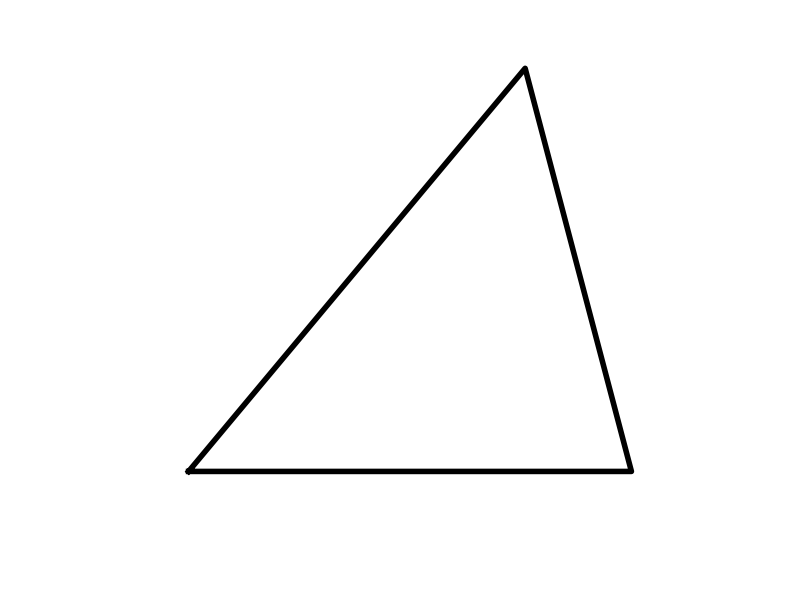
\includegraphics[width = \textwidth]{clip_figure0.png}
		\caption{初始三角面片}\label{subfig:clip0}
	\end{subfigure}
	\begin{subfigure}[b]{.32\textwidth}
		\centering
		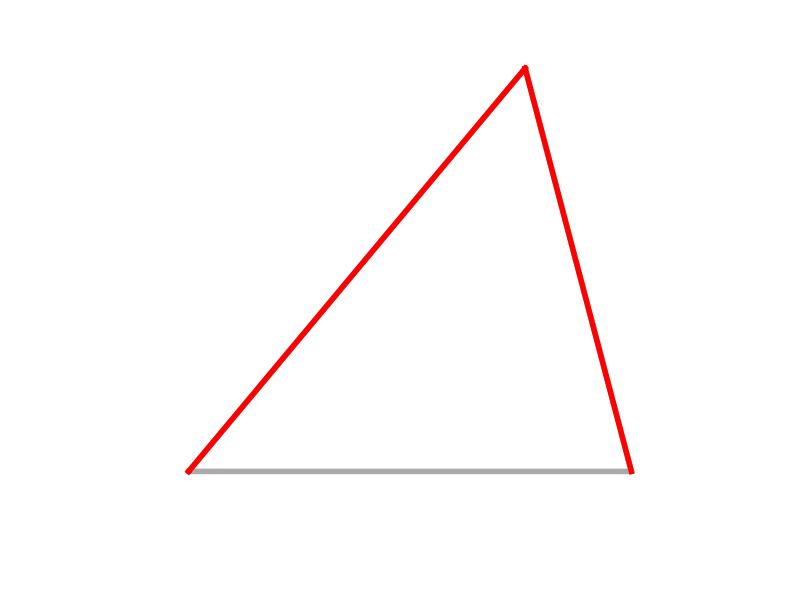
\includegraphics[width = \textwidth]{clip_figure1.png}
		\caption{初始三角面片}\label{subfig:clip1}
	\end{subfigure}
	\begin{subfigure}[b]{.32\textwidth}
		\centering
		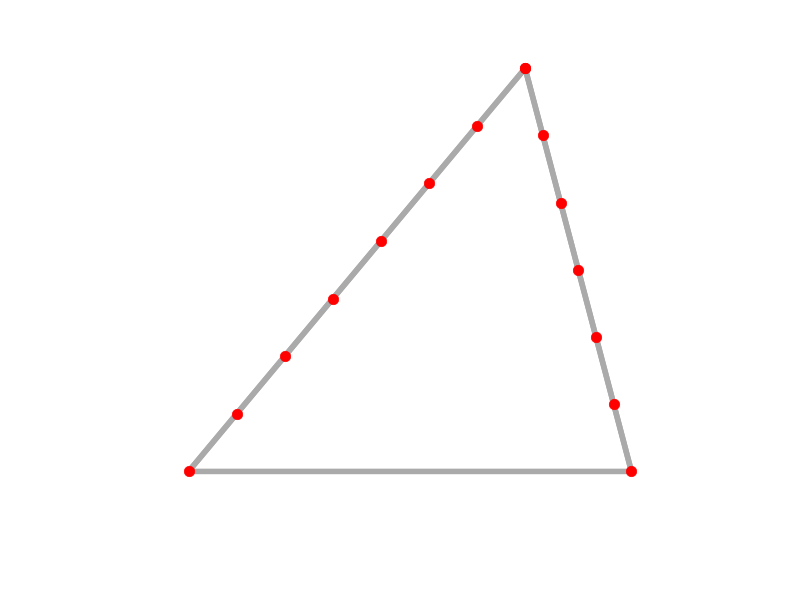
\includegraphics[width = \textwidth]{clip_figure2.png}
		\caption{分割最小角$\alpha$的两条边}\label{subfig:clip2}
	\end{subfigure}

	\begin{subfigure}[b]{.32\textwidth}
		\centering
		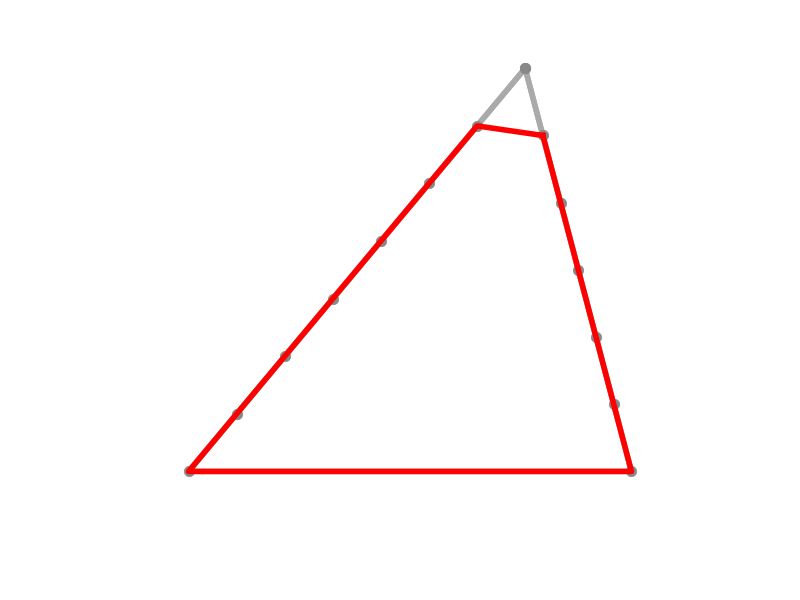
\includegraphics[width = \textwidth]{clip_figure3.png}
		\caption{切割第一个子三角形}\label{subfig:clip3}
	\end{subfigure}
	\begin{subfigure}[b]{.32\textwidth}
		\centering
		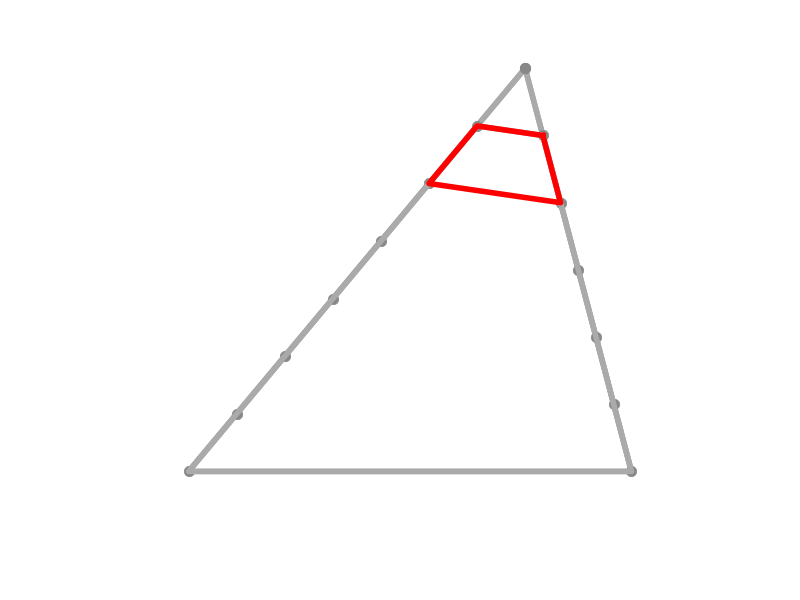
\includegraphics[width = \textwidth]{clip_figure4.png}
		\caption{第一个待分割层}\label{subfig:clip4}
	\end{subfigure}
	\begin{subfigure}[b]{.32\textwidth}
		\centering
		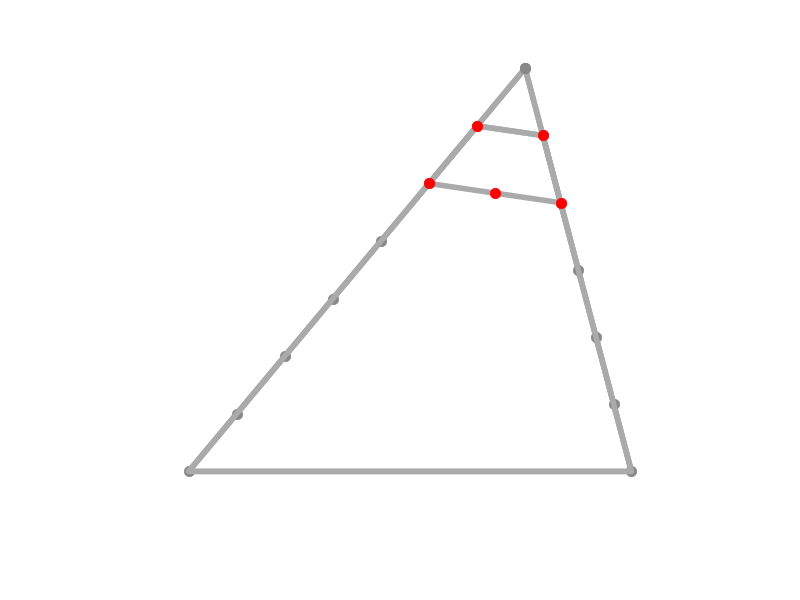
\includegraphics[width = \textwidth]{clip_figure5.png}
		\caption{分割待分割层的上下底边}\label{subfig:clip5}
	\end{subfigure}

	\begin{subfigure}[b]{.32\textwidth}
		\centering
		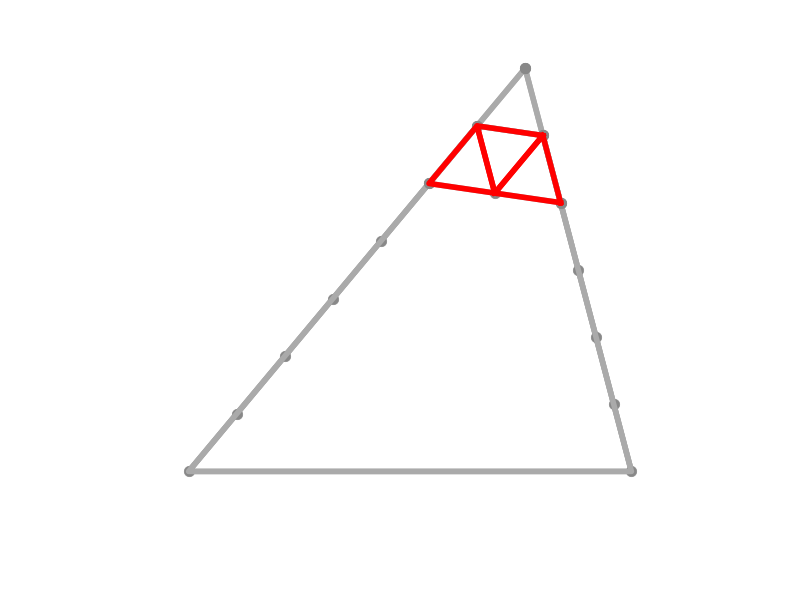
\includegraphics[width = \textwidth]{clip_figure6.png}
		\caption{分割待分割层的上下底边}\label{subfig:clip6}
	\end{subfigure}
	\begin{subfigure}[b]{.32\textwidth}
		\centering
		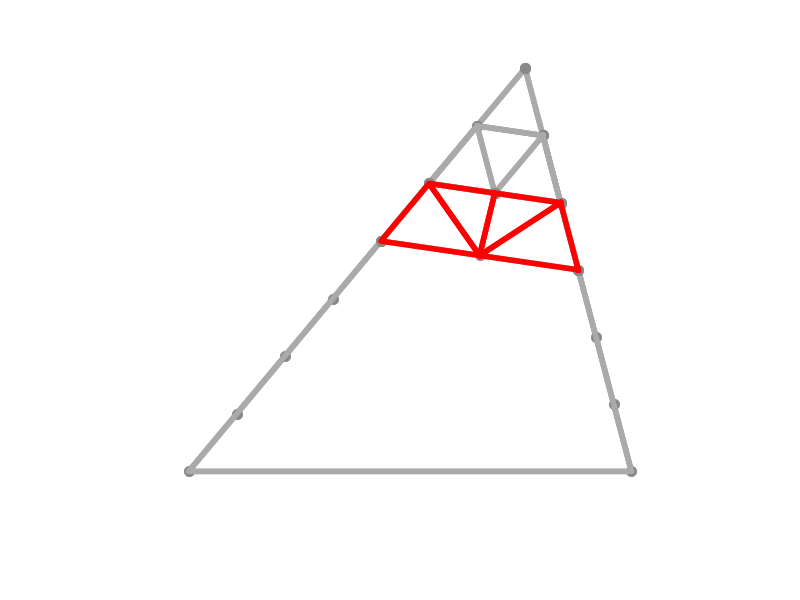
\includegraphics[width = \textwidth]{clip_figure9.png}
		\caption{分割待分割层的上下底边}\label{subfig:clip9}
	\end{subfigure}
	\begin{subfigure}[b]{.32\textwidth}
		\centering
		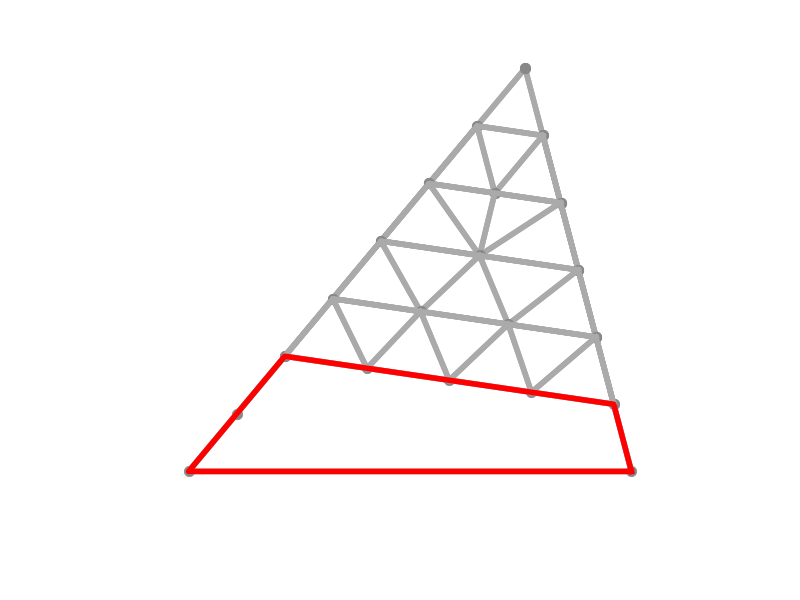
\includegraphics[width = \textwidth]{clip_figure16.png}
		\caption{继续分割红色部分}\label{subfig:clip16}
	\end{subfigure}

	\begin{subfigure}[b]{.32\textwidth}
		\centering
		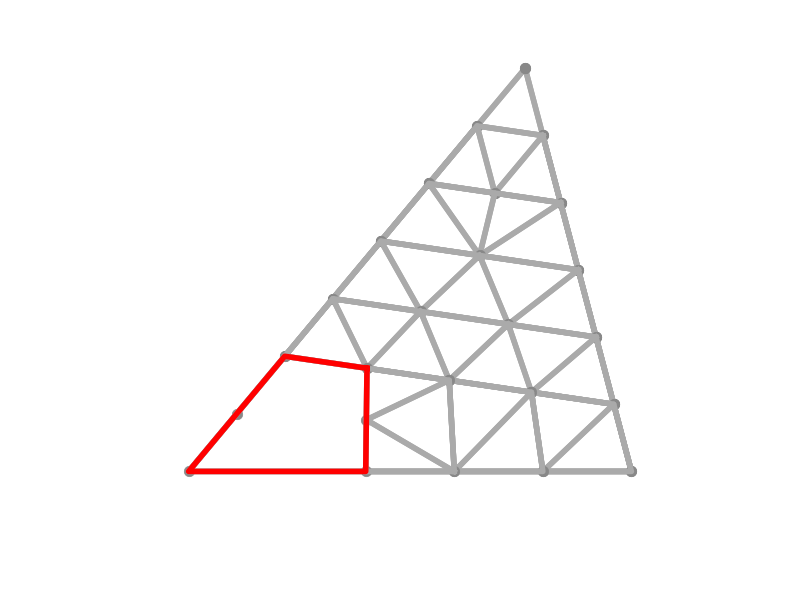
\includegraphics[width = \textwidth]{clip_figure26.png}
		\caption{对特殊情况进行处理}\label{subfig:clip26}
	\end{subfigure}
	\begin{subfigure}[b]{.32\textwidth}
		\centering
		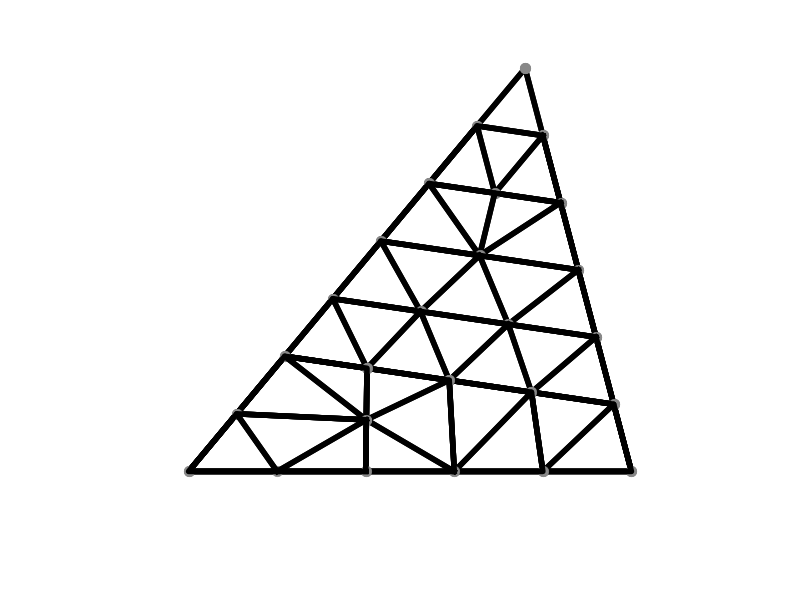
\includegraphics[width = \textwidth]{clip_figure33.png}
		\caption{分割结果}\label{subfig:clip33}
	\end{subfigure}
	\begin{subfigure}[b]{.32\textwidth}
		\centering
		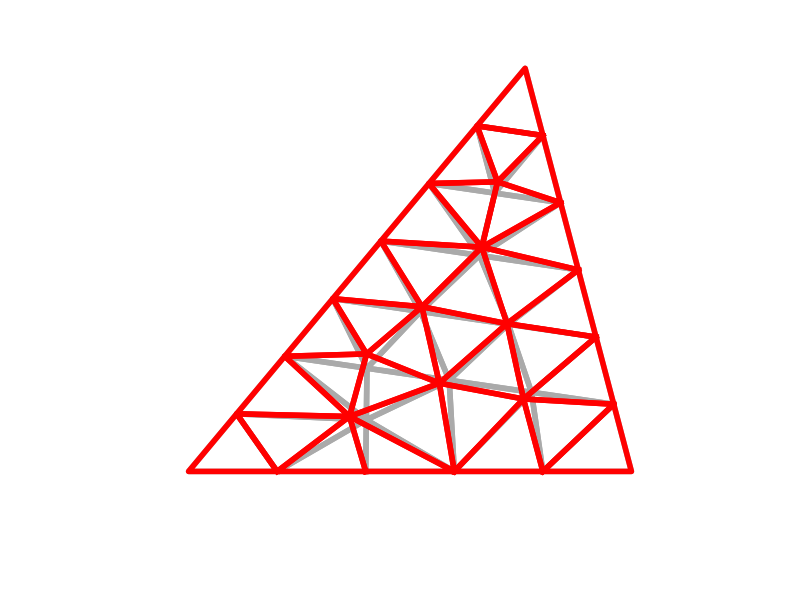
\includegraphics[width = \textwidth]{clip_figure34.png}
		\caption{对结果进行CVT优化}\label{subfig:clip34}
	\end{subfigure}
	\caption{均匀三角剖分算法}\label{fig:clip}
\end{figure}

CVT优化\cite{du1999}可以使分割更加均匀。且该过程可以迭代进行,使分割结果越来越均匀。\autoref{fig:CVT}展示了迭代过程,红色是优化之后的结果,灰色的是优化之前的。我们可以发现,从第5次迭代开始,每次迭代后的收益很小。所以我们最终选择对原始分割结果进行5次CVT迭代优化。

\begin{figure}[htbp]
	\centering
	\begin{subfigure}[b]{.49\textwidth}
		\centering
		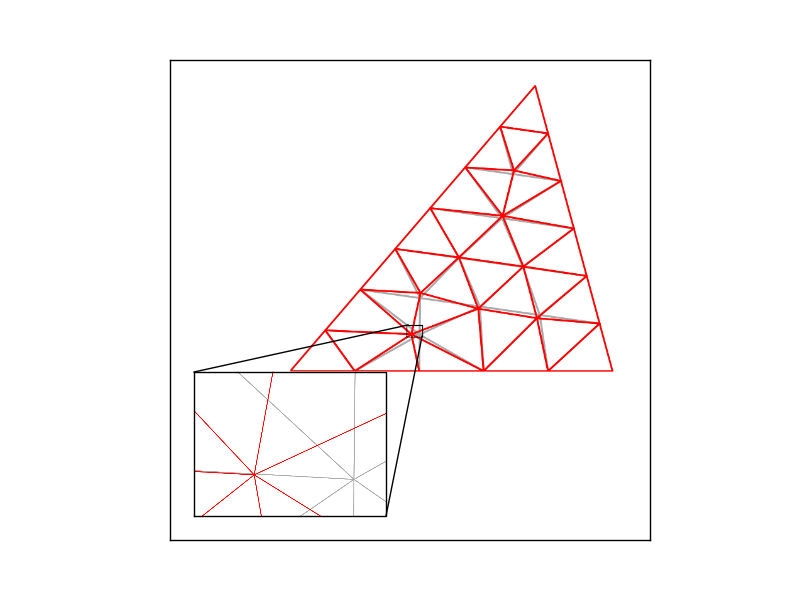
\includegraphics[width = \textwidth]{cvt_for_paper0.png}
		\caption{第1次CVT优化}
	\end{subfigure}
	\begin{subfigure}[b]{.49\textwidth}
		\centering
		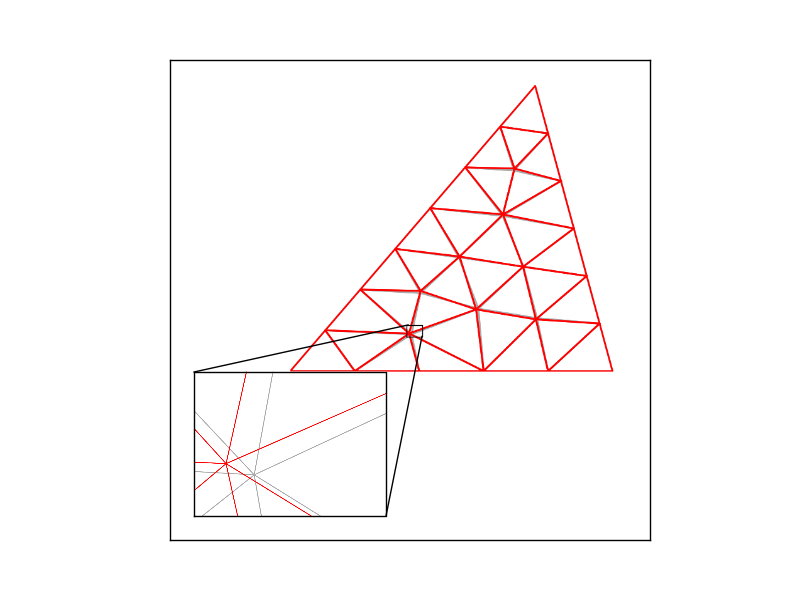
\includegraphics[width = \textwidth]{cvt_for_paper1.png}
		\caption{第2次CVT优化}
	\end{subfigure}

	\begin{subfigure}[b]{.49\textwidth}
		\centering
		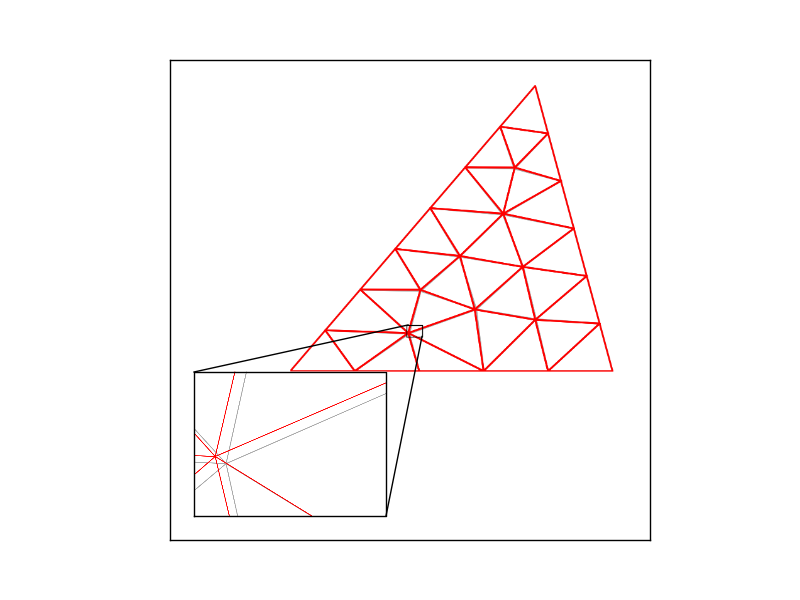
\includegraphics[width = \textwidth]{cvt_for_paper2.png}
		\caption{第3次CVT优化}
	\end{subfigure}
	\begin{subfigure}[b]{.49\textwidth}
		\centering
		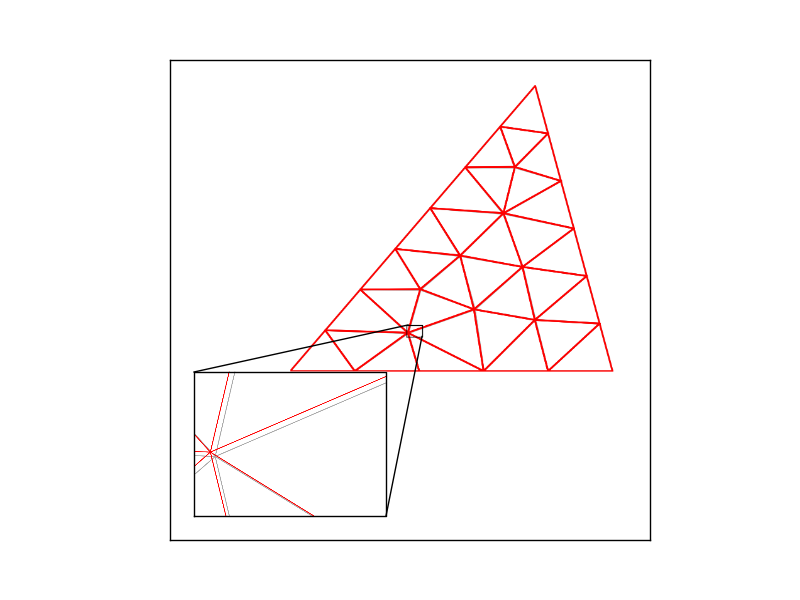
\includegraphics[width = \textwidth]{cvt_for_paper3.png}
		\caption{第4次CVT优化}
	\end{subfigure}

	\begin{subfigure}[b]{.49\textwidth}
		\centering
		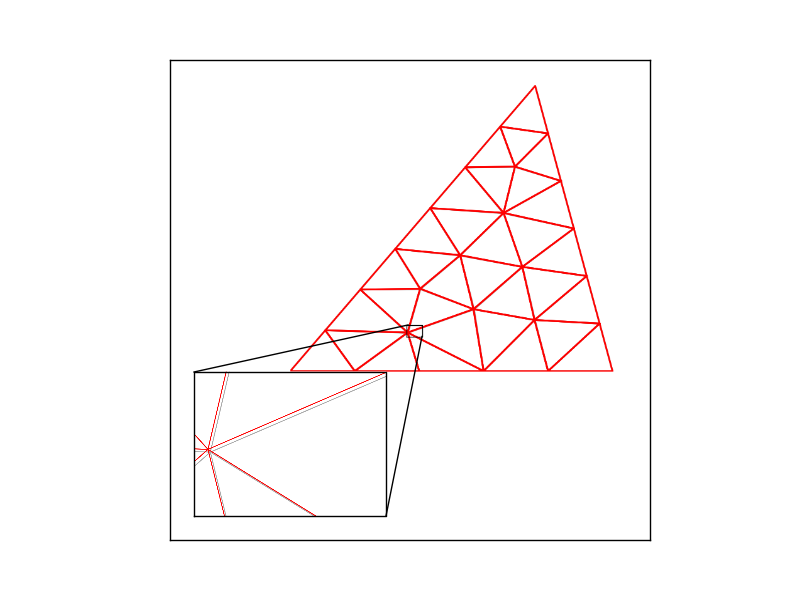
\includegraphics[width = \textwidth]{cvt_for_paper4.png}
		\caption{第5次CVT优化}
	\end{subfigure}
	\begin{subfigure}[b]{.49\textwidth}
		\centering
		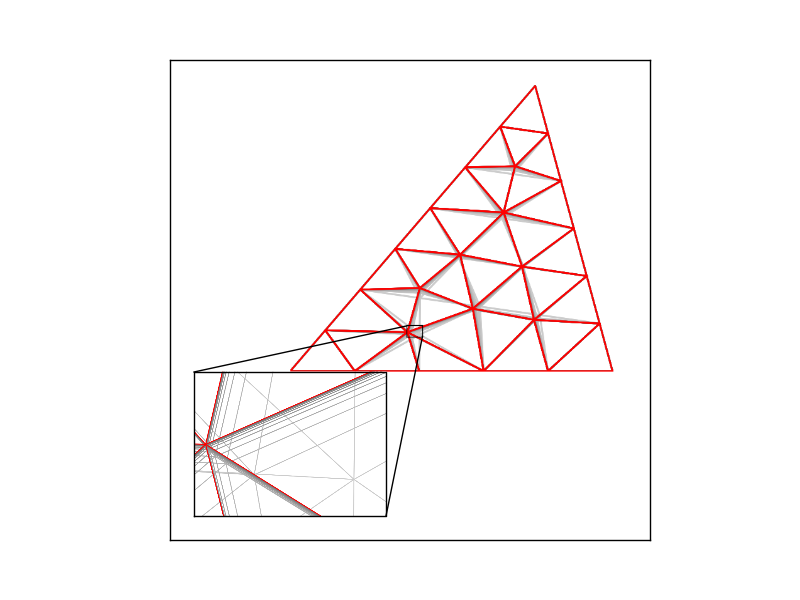
\includegraphics[width = \textwidth]{cvt_for_paper5.png}
		\caption{1~10次CVT优化}
	\end{subfigure}
    \caption{CVT优化结果} \label{fig:CVT}
\end{figure}

\section{关于$l$的讨论}
前文提到的$l$是一个很关键的参数,$l$不仅会影响算法效率、子三角形的质量\footnote{这里的质量表示接近正三角形的程度}、还能影响拟合得到的变形结果相对精确结果的拟合误差。但是,$l$并不是影响这些的根本因素,对分割后得到的子三角形的质量和算法效率产生直接影响的是子三角形的数目,而对变形结果的精度产生直接影响的是子三角形的平均面积\footnote{这两者在一定程度上是等价的,因为对于同一个三角形,剖分后得到的子三角形的数目趍,每个子三角形的面积就越小。}。$l$则通过改变子三角形数目或平均面积,间接地对算法效率、子三角形的质量、变形结果的精度产生影响。

定性的来说$l$越小,子三角形数目越多,面积越小,同时子三角形的质量越高,变形结果的误差越小,但算法的计算代价越高。为了进一步明确$l$对算法的影响,我们进行了一系列实验以定量的分析$l$。

实验选用了立方体模型,有12个面片,且模型被归一化到$[-1, 1]^3$。之所以选择由大三角面片组成的模型,是为了让三角面片随$l$变化切割出不同大小的子三角形。\autoref{fig:l-number}显示了$l$与子三角形数量的关系,蓝色表示以立方体为模型进行切割,立方体原始的三角面片平均面积为2.0;绿色表示以兔子玩偶为模型进行切割,兔子玩偶原始的三角面片平均面积为0.0007。从中我们可以发现由于兔子玩偶模型原始三角片面过小,当$l$大于某个值的时候,其不再被切割,子三角形的数目也保持不变,这样不利于我们探索$l$在变化过程中对变形算法产生的影响。而立方体由于原始三角面片较大,能随$l$变化切割出不同数目的子三角形。可以帮助我们更好的研究$l$对算法的影响。

变形空间的次数是$3\times3\times3$,控制顶点个数是$5\times5\times5$,变形空间范围是$[-1, 1]^3$。实验的自变量是$l$,由$0.1$增长到$2\sqrt{3}$\footnote{$2\sqrt{3}$为变形空间对角线长度}。因变量是算法效率、子三角形的质量和变形结果的精度。以下是实验结果。

%兔子模型的平均三角形面积为总表面积/三角形数目
%5.880918 / 8400 = 0.0007001092857142858
\begin{figure}[htbp]
	\centering
	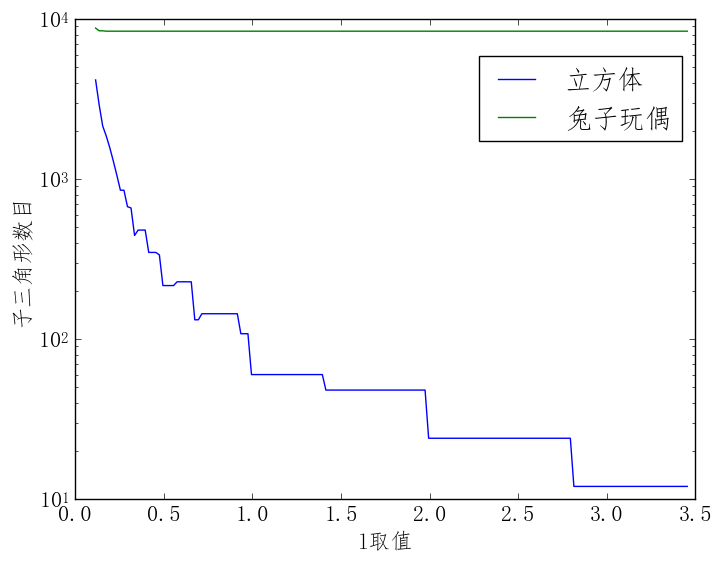
\includegraphics[width = 0.8\textwidth]{l-number.png}
	\caption{$l$取值-子三角形数目关系图}\label{fig:l-number}
\end{figure}

\subsection{算法效率}
从\autoref{fig:l-number}可以看出不同的$l$可能产生相同的分割结果,所以\autoref{fig:l-time0}中,$l$与算法运算时间的关系不是很直观。如前文所述,$l$通过影响子三角形数目,从而影响算法运算时间,所以我们直接探究子三角形数目和算法运算时间的关系。如\autoref{fig:l-time1}中所示,大体上来看,算法运行时间与子三角形数目呈线性正相关。

\begin{figure}[htbp]
	\centering
	\begin{subfigure}[b]{.45\textwidth}
	    \centering
	    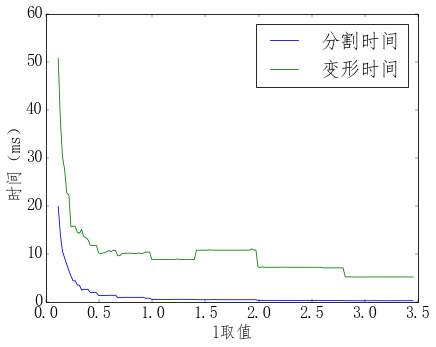
\includegraphics[width =\textwidth]{l-time0.png}
	    \caption{$l$取值-算法运行时间关系图}\label{fig:l-time0}
	\end{subfigure}
	\begin{subfigure}[b]{.45\textwidth}
	    \centering
	    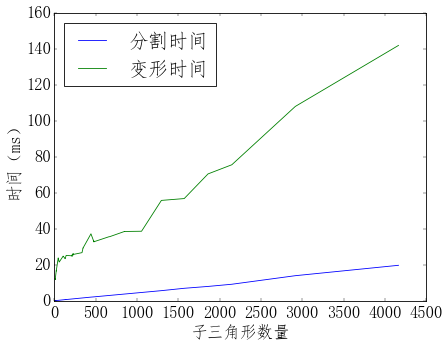
\includegraphics[width =\textwidth]{l-time1.png}
	    \caption{三角形数目-算法运行时间关系图}\label{fig:l-time1}
	\end{subfigure}
	\caption{$l$取值-算法效率}\label{fig:l-time}
\end{figure}

这部分数据说明当本文算法运行比较"卡"时,增加$l$值可以有效地加快算法响应速度。同时,可以指导用户根据硬件条件与编辑过程中对实时交互的依赖程度选择合适的$l$,如用户可以在编辑过程中选择较大的$l$,而在完成编辑,导出变形结果时选择较小的$l$,以兼顾精度和效率。

\subsection{子三角形质量}
    本节探讨$l$与子三角形质量之间的关系,在此之前,我们先明确本文中对于三角形质量的定义:三角形质量表示一个三角形从形状上接近正三角形的程度,三角形越接近正三角形,其质量越差,反之亦然。

    以上定义是对三角形质量定性的描述,我们需要进一步确定一个指标来衡量三角形的质量。有很多指标都可以衡量三角形质量\cite{pebay2003},我们选取了其中计算量较少的一个$q(t)=r_t/max(\{e_i\}^{2}_{i=0})$,即三角形外接圆的半径除以其最长边长度。该指标的取值范围是$(0, \frac{\sqrt{3}}{2}]$,当三角形$t$为正三角形时,$q(t)$取到最大值$\frac{\sqrt{3}}{2}$;三角形$t$越狭长,$q(t)$的值越接近0。为了更直观的用该指标表示三角形质量,我们修改将$q(t)$修改为$q(t)=r_t/max(\{e_i\}^{2}_{i=0})*2\sqrt{3}$,使其取值范围归一化到$(0, 1]$。\autoref{fig:triangle_quality_compare}可视化了两种三角形分割方法产生的三角形的质量,可以很明显的观察到沿节点盒切割方法生产的大量狭长三角形,而本文方法切割产生的三角形及其匀称。可见在这方面,本文方法明显占优。

\begin{figure}[htbp]
	\centering
	\begin{subfigure}[b]{.3\textwidth}
		\centering
		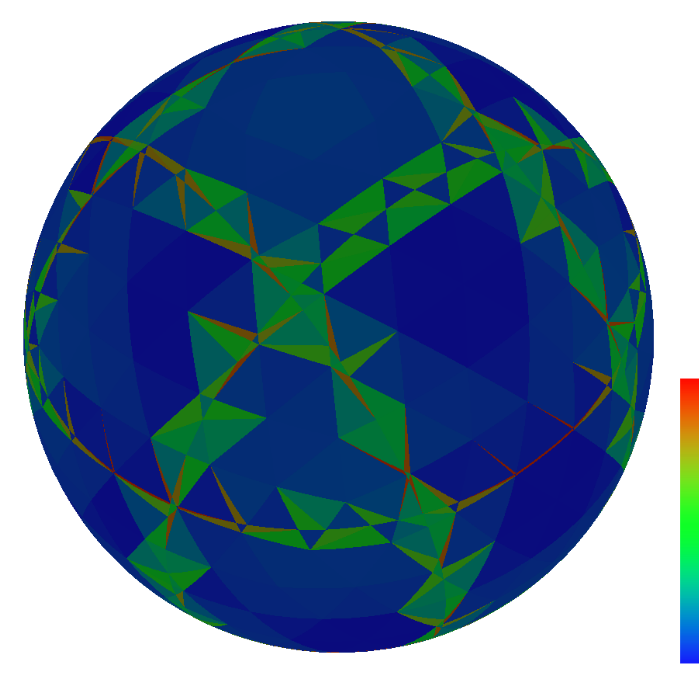
\includegraphics[width = \textwidth]{clip_compare0.png}
		\caption{沿节点盒切割}\label{subfig:clip_compare0}
	\end{subfigure}%
	\begin{subfigure}[b]{.3\textwidth}
		\centering
		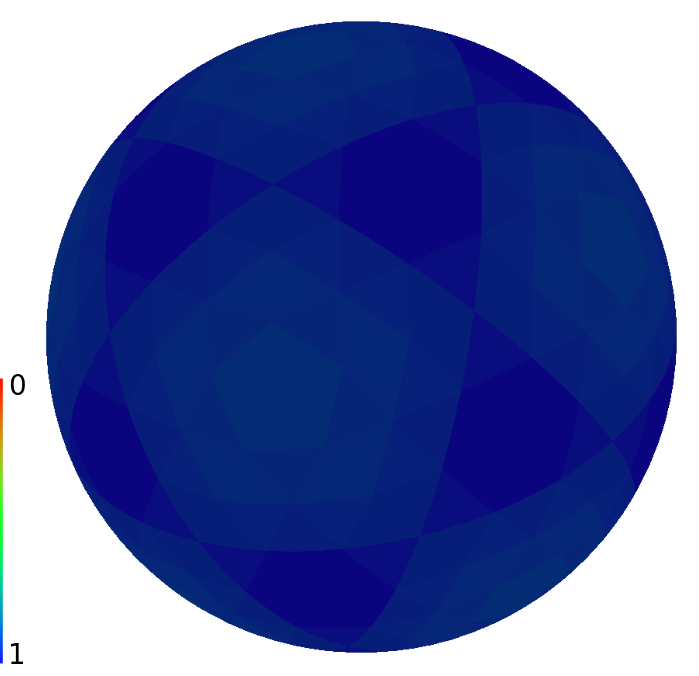
\includegraphics[width = \textwidth]{clip_compare1.png}
		\caption{本文方法}\label{subfig:clip_compare1}
	\end{subfigure}
	\caption{两种切割算法产生的子三角形的质量对比}\label{fig:triangle_quality_compare}
\end{figure}

不同的$l$对三角形质量的影响如\autoref{fig:l-quality}所示。我们分别作了$l$取值、子三角形数目与子三角形质量的关系图。可见$l$越小,三角形质量越高。但是由于切割算法中存在取整操作,所以\autoref{fig:l-quality}存在许多跳变的地方。同时我们可以从\autoref{subfig:l-quality1}中发现,当三角形数目达到某一临界值时,三角形质量不再显著增加。在该例子中这个值672,既每个原始三角形都被分成了56个小三角形。我们通过进一步实验发现,原始三角形的质量越差,该临界值就越大。

\begin{figure}[htbp]
	\centering
	\begin{subfigure}[b]{.45\textwidth}
		\centering
		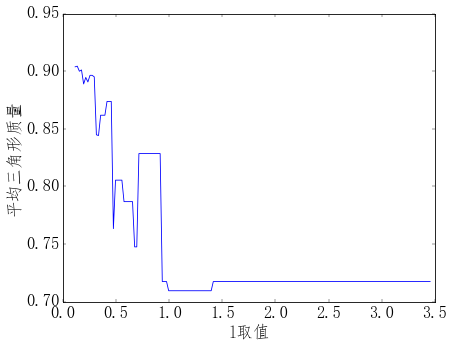
\includegraphics[width = \textwidth]{l-quality0.png}
		\caption{$l$取值-子三角形质量关系图}\label{subfig:l-quality0}
	\end{subfigure}%
	\begin{subfigure}[b]{.45\textwidth}
		\centering
		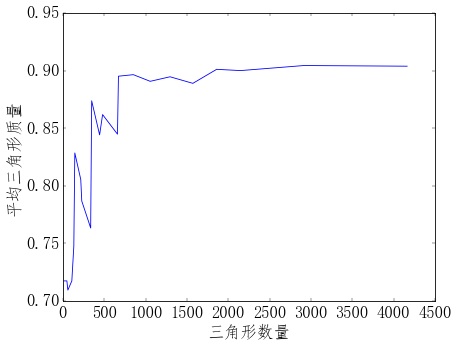
\includegraphics[width = \textwidth]{l-quality1.png}
		\caption{子三角形数目-子三角形质量关系图}\label{subfig:l-quality1}
	\end{subfigure}
	\caption{$l$取值-子三角形的质量对比}\label{fig:l-quality}
\end{figure}

\subsection{变形结果精度}
相比于光滑自由变形,本文方法会产生跨节点盒的子三角形。这些三角形会引入额外的误差。但是只要子三角足够小,误差就能控制在可接受范围内。我们同样做了实验以验证$l$取值与变形误差的关系。从\autoref{fig:l-error}中可以看出,变形结果的几何误差基本与子三角形面积呈线性正相关。
\begin{figure}[htbp]
	\centering
	\begin{subfigure}[b]{.45\textwidth}
		\centering
		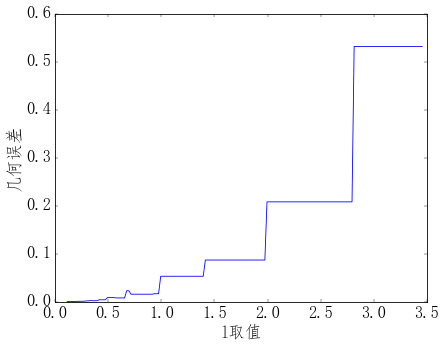
\includegraphics[width = \textwidth]{l-error0.png}
		\caption{$l$取值-子三角形质量关系图}\label{subfig:l-error0}
	\end{subfigure}%
	\begin{subfigure}[b]{.45\textwidth}
		\centering
		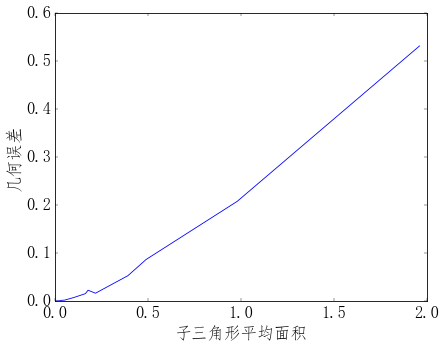
\includegraphics[width = \textwidth]{l-error1.png}
		\caption{子三角形数目-子三角形质量关系图}\label{subfig:l-error1}
	\end{subfigure}
	\caption{$l$取值-变形误差}\label{fig:l-error}
\end{figure}

\section{本章小结}
本章内容介绍了本文提出三角形均匀剖分算法的动机,用本文算法替换沿节点盒切割算法的可行性,本文算法的详细步骤以及本文算法的优势。除此之外,还讨论了三角形均匀剖分算法中参数$l$对于算法效率、剖分产生三角形的质量以及变形结果误差的影响。为用户选取合适的$l$提供了一定的指导。
